\chapter{IRK: Eguzki-sistema.}

\section{Sarrera.}

Koordenatu kartesiarrak erabiltzearen abantaila.

\section{Kepler-en fluxua.}
   
Kepler problema, bi gorputzen problemaren kasu partikularra da eta  honako Hamiltondarra dagokio,
\begin{equation}
H(p,q)=\frac{p^2}{2m}-\frac{\mu}{\|q\|},
\end{equation}
non $m$ eta $\mu$ konstanteen balioak, formulazioaren araberakoak diren.

Koordenatu sistema $q=q_2-q_1$ duen formulazioa aukeratzen badugu, konstanteen balioak hauek dira,  
\begin{equation*}
m=(1/m_1+1/m_2)^{-1},\ \ \mu=Gm_1m_2,
\end{equation*} 

eta ekuazio diferentzialak era honetan definitzen dira,
\begin{equation}
\dot{q}=p, \ \ \dot{p}= - \frac{k \ q}{\|q\|^3} ,
\end{equation}
non $k= \mu / m$ eta  $q,p \in \mathbb{R}^3$.

Kepler problemaren soluzio zehatza kalkula daiteke: une bateko kokapen eta abiadurak emanik, denbora tarte bat ($\Delta t$) igarotakoan (positiboa ala negatiboa), zehazki kokapen eta abiadura berriak ezagutu daitezke. Eguzki-sistemaren integrazio metodoentzat, Kepler problema doitasun handian eta era eraginkorrean konputatzea, funtsezkoa da. Kepler problemaren erreferentziazko inplementazioak, Danby \cite{Danby1992} eta J.Wisdom  \cite{Wisdom2015} ditugu. 

Kepler problemaren inplementazioaren lan egiteko modua, honakoa da. Lehenik, koordenatu cartesiarretatik ($q,p\in \mathbb{R}^3$), koordenatu eliptikoetara $(a,e,i,\Omega,E)$, itzulpena egingo dugu. Koordenatu eliptikoetan, $E$ (\emph{eccentric anomaly}) aldagaia izan ezik, beste aldagaiak konstante mantentzen dira: beraz $E_0$ balioa emanda, $\Delta t$ denbora tartea aurrera egin eta $E_1$ balioa berria kalkulatuko dugu. Azkenik, koordenatu eliptikoetatik koordenatu cartesiarretara itzulpena eginez, kokapen eta abiadura berriak eskuratuko ditugu. 

\begin{equation*}
(q_0,v_0) \in \mathbb{R}^6 \ \ \ \longrightarrow \ \ \  (a,e,i,\Omega,E_0) \in \mathbb{R}^6 
\end{equation*}
\begin{equation*}
\quad \quad \quad \quad \quad \quad \quad \quad \downarrow \Delta t
\end{equation*}
\begin{equation*}
(q_1,v_1) \in \mathbb{R}^6 \ \ \ \longleftarrow \ \ \  (a,e,i,\Omega,E_1) \in \mathbb{R}^6 
\end{equation*}

Inplementazioaren garapenaren zehaztasun guztiak eranskinaren \ref{erans:B1} atalean eman ditugu.
 


\section{Inplementazio berria.}

Eguzki sistemarako honako idei berri bat azalduko dugu. Honako ekuazio diferentziala dugularik,
\begin{equation*}
\dot{y}=k(y)+\epsilon \ g(y)
\end{equation*}

Alde kepleriarraren fluxua ezaguna dugu,
\begin{align*}
\varphi_{\triangle t}^k:&  \ \mathbb{R}^d \ \longrightarrow \mathbb{R}^d  \\
&  y_0 \longrightarrow y_1. 
\end{align*}

Aldagai aldaketa bat egin daiteke,
\begin{align*}
y(t_0+\triangle t) &= \varphi _{\triangle t}^k(z(t_0+\triangle t)), \ \ y(t_0)=z(t_0), \\
z(t_0+\triangle t) &= \varphi _{-\triangle t}^k(y(t_0+\triangle t)).
\end{align*}

Aldagai berriarekiko ekuazio diferentziala mantso aldatzen den funtzioa da,
\begin{align*}
\dot{z}=\epsilon \ r(z,t).
\end{align*} 

Ideia hau bi modutara aplika daiteke,
\begin{enumerate}
\item Gauss inplizituaren integrazio metodoan.
\item Atalen hasieraketa ona lortzeko.
Orokorrean, interpolazio bidezko hasieraketa ona izateko,  urratsa txikia izan behar du (periodo bat baino txikiagoa izan behar du). Teknika hau erabiliz, interpolazioaren errorea $\mathcal{O}(\epsilon)$ mailakoa izango da.

Proposamen honetan hasieraketa $z$ aldagai berria erabiliz era honetan egingo dugu:
\begin{itemize}
\item $Y_{n-1}$ atalei kepler \textbf{denboran atzeratuz}, $Z_{n-1}$ aldagai berriarekiko atalak lortuko ditugu.
\item $Z_{n-1}$ alatak interpolauz, $Z_{n}^{[0]}$ hasieraketak lortuko ditugu.
\item $Z_{n}^{[0]}$ atalei kepler \textbf{denboran aurreratuz}, $Y_{n}^{[0]}$ hasieraketak lortuko ditugu.
\end{itemize}


\end{enumerate}


\begin{figure}[!h]
\centering
\subfloat[Atalen hasieraketa1.]{
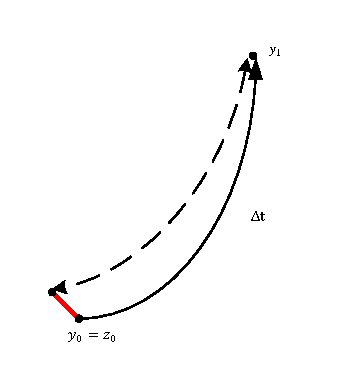
\includegraphics[width=.500\textwidth]{AtalenHasieraketa1}
}
\subfloat[Atalen hasieraketa2.]{
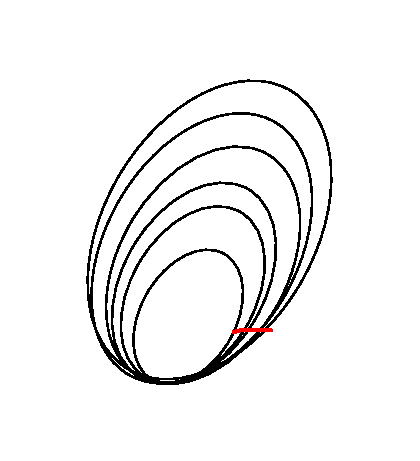
\includegraphics[width=.500\textwidth]{AtalenHasieraketa2}
}
\caption[Atalen hasieraketa.]
        {\small ....        
         \textbf{(a) irudian},                           
         \textbf{(b)} ......        
        }
\label{fig:Atalak12}
\end{figure}   

\begin{figure}[h]
\centerline{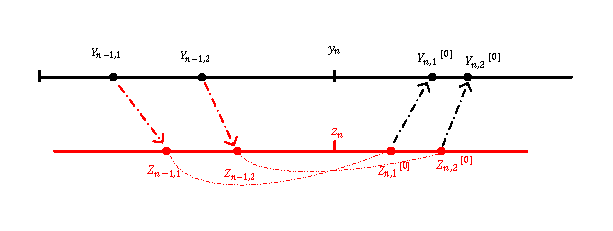
\includegraphics[width=12cm, height=6cm] {AtalenHasieraketa3}}
\caption{Atalen hasieraketa3.}
\label{fig:lau}
\end{figure} 


\section{Zenbakizko esperimentuak.}

\section{Laburpena.}